\documentclass[10pt,twocolumn,letterpaper]{article}

\usepackage{cvpr}
\usepackage{times}
\usepackage{epsfig}
\usepackage{graphicx}
\usepackage{amsmath}
\usepackage{amssymb}
\usepackage[lined,algonl,boxed]{algorithm2e}
\usepackage{algorithmic}

% Include other packages here, before hyperref.

% If you comment hyperref and then uncomment it, you should delete
% egpaper.aux before re-running latex.  (Or just hit 'q' on the first latex
% run, let it finish, and you should be clear).
\usepackage[pagebackref=false,breaklinks=true,letterpaper=true,colorlinks,bookmarks=false]{hyperref}

\newcommand{\todd}[1]{\textcolor{red}{[\bf TZ: #1]}}
\newcommand{\ruonan}[1]{\textcolor{blue}{[\bf RL: #1]}}

%\cvprfinalcopy % *** Uncomment this line for the final submission

\def\cvprPaperID{****} % *** Enter the CVPR Paper ID here
\def\httilde{\mbox{\tt\raisebox{-.5ex}{\symbol{126}}}}

% Pages are numbered in submission mode, and unnumbered in camera-ready
\ifcvprfinal\pagestyle{empty}\fi

\begin{document}

%%%%%%%%% TITLE
\title{Finding Group Interactions in Social Clutter}
\author{ Ruonan Li and Todd Zickler\\
Harvard School of Engineering and Applied Science\\
{\tt\small \{ruonanli,zickler\}@seas.harvard.edu}
}

\maketitle
% \thispagestyle{empty}

% !TEX root =  GroupDet.tex

\begin{abstract}
We consider the problem of finding distinctive social interactions involving groups of agents embedded within larger social gatherings. Given a pre-defined gallery of short exemplar interaction videos, and a long input video of a large gathering (with approximately-tracked agents), we identify within the gathering small sub-groups of agents exhibiting social interactions that resemble those in the exemplars. The participants of each detected group interaction are localized in space; the extent of their interaction is localized in time; and when the gallery of exemplars is annotated with group-interaction categories, each detected interaction is  classified into one of the pre-defined categories. Our approach represents group behaviors by dichotomous collections of descriptors for (a) individual actions, and (b) pair-wise interactions; and it includes efficient algorithms for optimally distinguishing participants from by-standers in every temporal unit and for temporally localizing the extent of the group interaction. Most importantly, the method is generic and can be applied whenever numerous interacting agents can be approximately tracked over time. We evaluate the approach using three different video collections, two that involve humans and one that involves mice.
\end{abstract}

%Participant information is accumulated over time through a voting scheme that provides insensitivity to tracking errors (e.g., broken tracks, false detections) as well as variations in the temporal extent of interaction. 
% !TEX root =  GroupDet.tex
\section{Introduction}

Social interactions are common, but they rarely take place in isolation. Conversations and other group interactions occur on busy streets, in crowded cafes, in conference halls, and in other types of social gatherings. In these situations, before a computer vision system can \emph{recognize} distinctive group interactions, it must first \emph{detect} them by distinguishing between participants and by-standers and by localizing them in time. This paper addresses this spatio-temporal detection problem for cases in which the actors in a large gathering can be reasonably detected and tracked.

\begin{figure}[t]
\begin{center}
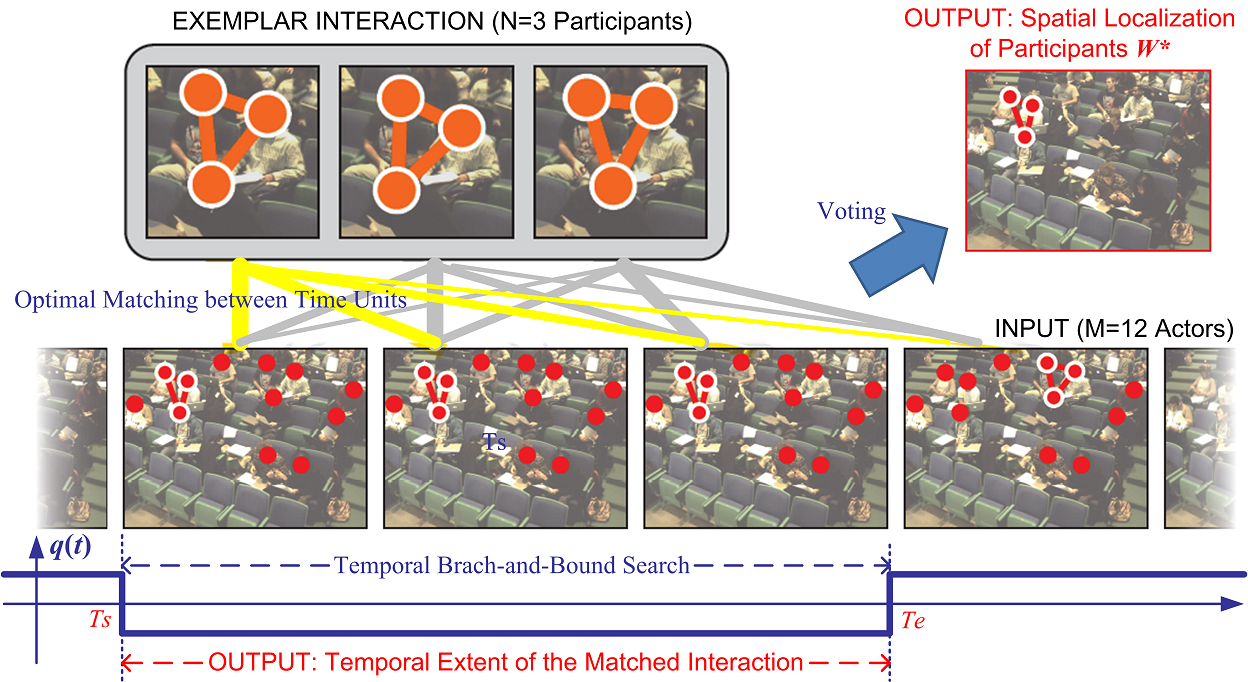
\includegraphics[width=\columnwidth]{diagram2.png}
\end{center}
\caption{Detecting and localizing interactions in social clutter. Given an exemplar video of an $N$-person social interaction, we seek to find similar interactions in a long input video with $M>N$ approximately-tracked actors. For each temporal frame in the exemplar, the $N$ best-matching participants are identified separately in each input video frame, and the matches are assigned scores. Matching scores are accumulated over time through Hough voting that is insensitive to tracking errors and changes in action rates, and this produces a spatial localization of the $N$ participating actors. Their interaction is then localized in time using an efficient branch-and-bound search.}
\label{diagram}
\end{figure}

We consider group interactions broadly as any distinctive space-time structural co-occurrence of individual actions, which occur in a variety of places and over a variety of times scales. We might want to find at a cocktail party, for example, all three-person conversations dominated by one person for a sustained period of time. On a busy street, we could search for all cases in which two passersby exchange a ``hello''. In a collection of hockey games, we might want all instances of a ``three-on-one'', and in nature we might be interested in localizing instances of distinctive group interactions among populations of animals, insects, or bacteria. Each of these cases would likely require distinct algorithms for detecting and tracking the actors, and each would benefit from action descriptors that are tuned for that setting. But beyond this, all of these scenarios can be abstracted as collections of (possibly fragmented and noisy) trajectories with accompanying time-varying action descriptors, and this is the abstraction on which we operate.
 
As depicted in Fig.~\ref{diagram}, our approach is based on matching. Given an exemplar video of a distinctive group interaction involving a small handful ($N$) of people, we aim to detect and localize instances of similar interactions within a long video of a larger gathering (\ie, of $M\ge N$ people). We represent a group interaction as an ensemble of two types of time-varying descriptors: per-actor descriptors that encode the appearance and/or motion of each participant, and relative pairwise descriptors that encode the appearance and/or motion of each participant relative to another. Matching an exemplar interaction then amounts to searching through space and time for ensembles that are similar in some sense. This approach avoids generating explicit semantic descriptions of group interactions, and it is advantageous when one lacks the vocabulary to precisely describe a class of interactions, or when they cannot easily be broken down according to any pre-defined grammar. To use our matching approach for recognition, we simply match an input video against a labeled gallery of exemplars and then extract a class label or ranked list of labels from the resulting scored matches.

In designing our detection system we face two main challenges. First, we expect tracks to be fragmented and noisy, and we expect the presence of outlying fragments caused by false detections, so we want an approach that can succeed in spite of these. Second, we expect that the same type of interaction can occur over different temporal extents, and at variable rates within its temporal extent, so we want an approach that is insensitive to these ``within-class'' variations. We address these challenges using a voting-based approach, which is depicted in Fig.~\ref{diagram}. First, the social descriptor-ensemble at each exemplar time frame is compared separately to each frame of the input video, and the best-matching $N$ participants in each frame are identified along with their matching score (yellow and gray lines in Fig.~\ref{diagram}). Second, weighted votes are accumulated from these frame-wise matches to obtain a final estimate of the $N$ participants. Third and finally, the temporal extent of the interaction is determined through an efficient branch-and-bound search. Our designs for these three processing stages are tightly connected to each other and to our representation for interactions. Optimal frame-wise matching is made possible by our restriction to second order (individual and pairwise) action descriptors, and a large-margin-based metric learning procedure serves the dual role of improving voting (step two) and enabling efficient branch and bound search (step three).

Previous work on action detection mostly consider actions of a single actor~\cite{Ke:detection,Yuan:detection,Shechtman:detection,Hu:detection,Laptev:detection,Duchenne:detection}. Previous work on group activity recognition 1) both assume an input video to be temporally cropped around one group activity and assume no by-standers \cite{Intille:act,Ni:group,Lan:Group}; 2) only account for temporal localization \cite{Hongeng:act,Gong:act,Hakeem:act,McCowan:meeting,Choi:recogtrack,Vlad:group, Ryoo:group, CRIM13}; or 3) only consider identifying participants \cite{Li:segmentation,Cristani:discovery}. \cite{Amer:group}  addresses a similar problem to ours but with less flexible representations of social interactions (more on this in Section~\ref{expall}). 

We evaluate our approach using three very different datasets: 1) the UT-Interaction Dataset~\cite{Ryoo:group}; 2) a new collection of videos from an `interactive classroom' (e.g.~\cite{Crouch:PI}) in which students self-organize in small group discussion; and 3) the Caltech Resident-Intruder Mouse dataset \cite{CRIM13}.



%Each detected instance of interaction is spatially localized in that the $N$ participants are distinguished from the $M-N$ bystanders and explicitly identified with the participants in the exemplar video. Each detected instance is also temporally localized by inferring the exact times in which the interaction begins and ends. 
%So our approach operates primarily in the space of tracklets, with a critical design criteria being insensitivity to tracking errors (\eg, broken tracks and false tracklets) in the input video.

%Our work builds on a small collection of related work: \cite{Li:segmentation} identifies the relevant motion from a clutter, \cite{Cristani:discovery} detects pre-defined geometric configuration of individual poses, and \cite{Lan:retrieval} retrieves individual actions in the context of surrounding humans. Those more similar to ours are \cite{Ryoo:group,Amer:group}: The former recognizes and temporally localizes interactions, and the latter implicitly infers participants from a generative model for a set of histograms of pose-coded detections computed at a dense spatio-temporal grid. We empirically compare our approach with \cite{Ryoo:group,Amer:group} in Section \ref{expall}.


%In a round-table discussion, we could find intervals where one speaker holds the attention of her neighbors for some extended time. 
%\section{Matching and Localizing Social Interactions}


Consider an input video consisting of $T$ temporal units, with each unit being a frame or several consecutive frames. By applying domain-appropriate detection and tracking, assume we obtain $M$ space-time tracks of bounding boxes enclosing $M$ faces or bodies. Note that these $M$ tracks may include non-participants and false-alarm bounding boxes resulted from an imperfect detector. The $M$ targets are to be compared with the social interaction exemplars pre-stored in a database. Such an exemplar consists of $S$ temporal units and $N$ targets that are correctly detected and tracked and all participating in an coherent social interaction. As the input may include non-participants and false-positive tracks, it contains the same or more targets than the exemplar, \textit{i.e.}, $N\leq M$.

The first question is how to represent the two sets of size $M\times T$ and $N\times S$. A social interaction is not only a collection of individual activities, but is more crucially characterized by the mutual contexts between individuals. Our representation for the input tracks is consequently made up of two parts. The first part is a collection of $M\times T$ $d_{I}$-dimensional descriptors $\{\mathbf{f}_{m,t}\}_{m=1,2,\cdots,M, t=1,2,\cdots,T}$, where $\mathbf{f}_{m,t}$ encodes the individual activity of the $m$th target at time $t$. The other part is a collection of $M\times (M-1)\times T$ $d_{P}$-dimensional pairwise contextual descriptors $\{\mathbf{g}_{m,m',t}\}_{m,m'=1,2,\cdots,M, m\neq m', t=1,2,\cdots,T}$, where $\mathbf{g}_{m,m',t}$ encodes dynamic visual properties of target $m$ that are exhibited relative to those of target $m'$ at time $t$. Loosely speaking, $\mathbf{g}_{m,m',t}$ describes the `influence' that target $m'$ exhibits over target $m$ at time $t$, with the possibility that $\mathbf{g}_{m,m',t}\ne\mathbf{g}_{m',m,t}$. The form of descriptors $\mathbf{f}_{m,t}$ and $\mathbf{g}_{m,m',t}$ will be application dependent, and will be further discussed in experiment section. For each exemplar, we have two similar descriptor collections $\{\mathbf{f}^{D}_{n,s}\}_{n=1,2,\cdots,N, s=1, 2,\cdots, S}$ and $\{\mathbf{g}^{D}_{n,n',s}\}_{n,n'=1,2,\cdots,N, n\neq n', s=1, 2,\cdots, S}$. We denote the descriptor ensemble for the input at time $t$ to be $\mathcal{Q}_{t}\triangleq\{\mathbf{f}_{m,t},\mathbf{g}_{m,m',t}\}$, and that for the exemplar at time $s$ as $\mathcal{D}_{s}\triangleq\{\mathbf{f}^{D}_{n,s},\mathbf{g}^{D}_{n,n',s}\} $. As a result, the input can be represented as $\mathcal{Q}\triangleq\{\mathcal{Q}_{t}\}_{1\leq t\leq T}$ and the exemplar $\mathcal{D}\triangleq\{\mathcal{D}_{s}\}_{1\leq s\leq S}$.


Given the input and the exemplar, our primary tasks are to identify from the $M$ targets in the input $N$ targets that demonstrate the most similar socially interactive pattern as the $N$ individuals in the exemplar, as well as to temporally localize the extent of the interaction within the interval $[1, T]$. To formally describe the former task, consider the fact that if one of the $M$ targets is regarded as a participant in an interaction as exemplified by the exemplar $\mathcal{D}$, its behavior should properly match to the behavior of one of the $N$ individuals in the exemplar $\mathcal{D}$. Therefore, we use a $N\times M$ binary matrix $W=[w_{nm}]\in\{0,1\}^{N\times M}$ to formally represent the participant identification, where $w_{nm}=1$ means that the $n$th exemplar individual is matched to the $m$th input target and $w_{nm}=0$ means unmatched targets. For unambiguous matching, we expect each individual in the exemplar to find its unique partner target in the input. This implies that $\sum_{m}w_{nm}=1, \forall n$ and $\sum_{n}w_{nm}\leq 1, \forall m$, \textit{i.e.}, $W\mathbf{1}=\mathbf{1}$ and $\mathbf{1}^{T}W\leq\mathbf{1}^{T}$\footnote{Note that false-alarm tracks are already accounted for in the partial matching, and if we set the values of the descriptors of an out-of-scene target to be sufficiently large (or small) numbers, this target will not be matched with any target in the exemplar.}. Denote $\mathcal{W}\triangleq\{W\in\{0,1\}^{N\times M}| W\mathbf{1}=\mathbf{1}, \mathbf{1}^{T}W\leq\mathbf{1}^{T}\}$, and our former task is essentially to find $W^{*}\in\mathcal{W}$, which encodes the best matching between the input $\mathcal{Q}$ and the exemplar $\mathcal{D}$. To formally describe the latter task is straightforward: We simply look for the starting time $T_{s}$ and ending time $T_{e}$, $1\le T_{s}<T_{e}\le T$, such that the interactive pattern of input $\mathcal{Q}$ during $[T_{s}, T_{e}]$ demonstrate the best similarity with the exemplar $\mathcal{D}$.

Our computational framework has three steps as illustrated in Figure \ref{diagram}. The first step is to evaluate $T\times S$ dis-similarity scores $D(\mathcal{Q}_{t}, \mathcal{D}_{s})$ together with their 'instantaneous optimal matching' $W^{t,s}$ between each time unit  $1\le t\le T$ and each time unit  $1\le s\le S$ (Section \ref{agg}). This is followed by a dual-accumulator Hough voting procedure to find the best matching $W^{*}$ (Section \ref{vote}). Finally, an efficient branch-and-bound search estimates the temporal extent $[T_{s}, T_{e}]$ (Section \ref{BB}).  
% !TEX root =  GroupDet.tex
\section{Matching and Localization of Interactions}

\vspace{-5pt}

\subsection{Representation}

\vspace{-5pt}

We consider a video as a sequence of $T$ temporal units that occur at a frequency equal to or less than the frame-rate of the raw video data. The duration of these $T$ units is typically between one and a  few raw video frames, and it is determined by one's application-appropriate choice for temporal resolution of computing atomic action descriptors (e.g., positions, velocities, accelerations, histograms of flow, space-time SIFT). We assume the existence of an application-specific detection and tracking system that outputs $M$ space-time tracks, which can be time-varying points, bounding boxes, silhouettes, or something else. Due to agent entry and exit, occlusions, and other tracking errors, not all $M$ tracks will persist over all $T$ frames, and some of the $M$ tracks may correspond to short-lived false detections.  The value of $M$ is thus the total number of trajectory fragments that are identified with distinct agents.

With each track we associate ensembles of two types of descriptors. There are $TM$ per-time-unit $d_{I}$-dimensional descriptors $\{\mathbf{f}_{m,t}\}$ where $\mathbf{f}_{m,t}$ encodes the $m$th agent's activity at time unit $t\in[1, T]$; and $TM(M-1)$ pairwise $d_{P}$-dimensional descriptors $\{\mathbf{g}_{m,m',t}\}$ where $\mathbf{g}_{m,m',t}$ encodes at time $t$ the motion and/or appearance of agent $m$ relative to agent $m', m'\ne m$. Loosely speaking, $\mathbf{g}_{m,m',t}$ captures the ``influence'' that agent $m'$ has over agent $m$ at time $t$. This influence is not symmetric in general, so typically $\mathbf{g}_{m,m',t}\ne \mathbf{g}_{m',m,t}$.  We use the notation $\mathcal{Q}_{t}\triangleq\{\mathbf{f}_{m,t},\mathbf{g}_{m,m',t}\}$ for the ensembles of all $M$ tracks at time $t$, and $\mathcal{Q}\triangleq\{\mathcal{Q}_{t}\}_{1\leq t\leq T}$ for the ensembles harvested from the entire input video. As mentioned above, the dimensions and entries in the descriptor vectors $\mathbf{f}$, $\mathbf{g}$ will be application dependent, and we consider a variety of examples in our experiments.

Each exemplar video is processed in the very same way as the input video, so that an exemplar of $N\le M$ participants over $S$ time units is represented at each time $s\in [1,S]$ by the ensemble $\mathcal{D}_{s}\triangleq\{\mathbf{f}^{D}_{n,s},\mathbf{g}^{D}_{n,n',s}\}$. We use the analogous notation $\mathcal{D}\triangleq\{\mathcal{D}_{s}\}_{1\leq s\leq S}$ for the ensembles collected from the entire exemplar. 

\vspace{-5pt}
\subsection{Matching between Temporal Units}

\label{agg}
\vspace{-5pt}

The first step in our framework is to separately compute the correspondence between the $N$ exemplar agents at each time $s\in[1, S]$ and the optimal subset of $N\le M$ of input agents at each time $t\in[1, T]$. We represent this $N$-to-$M$ correspondence by the $N\times M$ binary matrix $W$, where the $nm$-th entry $w_{nm}$ is one only when the $n$th exemplar agent is matched to the $m$th input agent.\footnote{Missing input tracks at time $t$ are handled by setting the values of the missing descriptors to be sufficiently large (or small) so as not to be matched with any agents in the exemplar.} Matches must be unique, so these matrices must have one non-zero entry in each row and at most one non-zero entry in each column: $W\mathbf{1}=\mathbf{1}$ and $\mathbf{1}^{T}W\leq\mathbf{1}^{T}$. We use the symbol $\mathcal{W}$ to represent the space of all such matrices, \ie, $\mathcal{W}\triangleq\{W\in\{0,1\}^{N\times M}| W\mathbf{1}=\mathbf{1}, \mathbf{1}^{T}W\leq\mathbf{1}^{T}\}$.

The quality of a correspondence is measured by the similarity between the individual and pairwise descriptors of the $N$ selected input agents and those of the $N$ exemplar agents. We formalize this by defining 
\begin{equation}
\vspace{-10pt}
\begin{split}
&\hat{D}(\mathcal{Q}_{t}, \mathcal{D}_{s}, W)=\\
&\sum_{nm}w_{nm}d_{I}(\mathbf{f}_{m,t}, \mathbf{f}^{D}_{n,s})+\!\!\!\!\!\!\sum_{nmn'm'}\!\!\!\!\!w_{nm}w_{n'm'}d_{P}(\mathbf{g}_{m,m',s}, \mathbf{g}^{D}_{n,n',t}),
\end{split}
\vspace{-10pt}
\end{equation}
to be the dissimilarity between two instantaneous ensembles under a particular matching matrix $W$. We use Mahalonobis distances to compare descriptors in this expression, so that $d_{I}(\mathbf{f}, \mathbf{f}')=(\mathbf{f}-\mathbf{f}')^{T}\Sigma_{I}(\mathbf{f}-\mathbf{f}')$ and $d_{P}(\mathbf{g}, \mathbf{g}')=(\mathbf{g}-\mathbf{g}')^{T}\Sigma_{P}(\mathbf{g}-\mathbf{g}')$, with $\Sigma_{I}\succeq 0$ and $\Sigma_{P}\succeq 0$ positive semi-definite matrices learned from exemplar videos as will be described in Sec.~\ref{MetLearn}.

Our immediate objective is to find the matching matrix $W\in\mathcal{W}$ that minimizes the score $\hat{D}(\mathcal{Q}_{t}, \mathcal{D}_{s}, W)$. Letting $\mathbf{w}$ be the vector formed by stacking the columns of $W$, the optimization can be expressed as
\begin{equation}
\label{Prob1}
\min_{w_{nm}\in\{0,1\}}\mathbf{c}^{T}\mathbf{w}+\mathbf{w}^{T}H\mathbf{w},\ \ \textup{s.t.}\ W\mathbf{1}=\mathbf{1}, \mathbf{1}^{T}W\leq\mathbf{1}^{T},
\end{equation}
where $\mathbf{c}$ is a $MN\times 1$ vector of distances between individual descriptors, $d_{I}(\mathbf{f}_{m,t}, \mathbf{f}^{D}_{n,s})$, and $H$ is a $MN\times MN$ matrix of distances between pairwise descriptors $d_{P}(\mathbf{g}_{m,m',t}, \mathbf{g}^{D}_{n,n',s})$'s. This problem has integer constraints and is generally not convex, so we instead solve
\begin{equation}
\label{Prob2}
\min_{w_{nm}\in[0,1]}(\mathbf{c}+\hat{\mathbf{c}})^{T}\mathbf{w}+\mathbf{w}^{T}(H+\hat{H})\mathbf{w}, \textup{s.t.} W\mathbf{1}=\mathbf{1}, \mathbf{1}^{T}W\leq\mathbf{1}^{T},
\end{equation}
where $\hat{\mathbf{c}}=[\sigma_{1},\sigma_{2},\cdots,\sigma_{MN}]^{T}$, $\hat{H}=\text{diag}\{-\sigma_{1},-\sigma_{2},\cdots,-\sigma_{MN}\}$, and each $\sigma_{i}$ is a sufficiently large number greater than $\sum^{MN}_{j=1,j\neq i}|H_{ij}|+H_{ii}$. 

Note that $\hat{H}$ imposes a negative strictly dominant diagonal to $H$ and the quadratic term $\hat{H}+H$ is strictly negative definite. Therefore, (\ref{Prob2}) is a concave programming in the convex unit hypercube $[0,1]^{N\times M}$ and will achieve its minimum at one of the feasible vertices. The feasible vertices, meanwhile, are exactly the feasible solutions of (\ref{Prob1}), and at these vertices, the values of the objective of (\ref{Prob2}) are equal to those of (\ref{Prob1}) due to the cancellation brought by $\hat{\mathbf{c}}$. It is therefore implied that by solving the much more efficient Problem (\ref{Prob2}) we obtain the exact solution for the original Problem (\ref{Prob1}). We solve (\ref{Prob2}) using the CVX toolbox \cite{cvx}.

Denote $D(\mathcal{Q}_{t}, \mathcal{D}_{s})\triangleq\min_{W\in\mathcal{W}}\hat{D}(\mathcal{Q}_{t}, \mathcal{D}_{s}, W)$ and $W^{t,s}\triangleq\arg\min_{W\in\mathcal{W}}\hat{D}(\mathcal{Q}_{t}, \mathcal{D}_{s}, W)$, and it is evident that $D(\mathcal{Q}_{t}, \mathcal{D}_{s})$ describes how similar the instantaneous interaction of input at time $t$ is to the instantaneous interaction of exemplar at time $s$, and $W^{t,s}$ encodes which $N$ of the $M$ agents in the input at time $t$ are selected to optimally match to the $N$ agents in the exemplar at time $s$ for yielding the value $D(\mathcal{Q}_{t}, \mathcal{D}_{s})$.


\subsection{Voting for Participant Identification}
\label{vote}

The second step of our framework is to identify $N$ agents from the $M$ input agents who \emph{overall} exhibit the maximal similarity with the $N$ exemplar agents. Let us denote this overall optimal correspondence by matching matrix $W^{*}\in\mathcal{W}$.  As $W^{*}$ specifies $N$ targets which demonstrate a consistently similar interactive pattern as the exemplar $\mathcal{D}$ over a substantial period in the input $\mathcal{Q}$, if we compute the instantaneous optimal matching $W^{t,s}$ for all $t$ and all $s$, the overall optimal matching $W^{*}$ will emerge many times among all computed $W^{t,s}$s. In other words, the desired $W^{*}$ will be supported by a large number of optimal instantaneous matchings. 

The scenario now resembles the settings for a general Hough Transform, where the desired parameters are supported by the maximum number of image feature observations: A parameter set and an observation set are established, for every observation one enumerates over all parameters and determines every parameter that is compatible with the observation, the count for that compatible parameter in an accumulator array for all parameters is increased by one, and finally the parameter receiving the maximum number of counts is reported. Here, we regard the parameter set as consisted of two parts - the set of all possible matchings $\mathcal{W}$ and the exemplar $\mathcal{D}$, and we regard the observation set as the input $\mathcal{Q}$. However, note that the overall optimal matching may not simply be achieved on the matching receiving the maximum number of counts, but on the matching which yields the maximum similarity with the exemplar. Therefore, in addition to maintaining an accumulator array for the counts on all matchings $\mathcal{W}$, we also maintain a companion accumulator array for the corresponding dissimilarity measures achieved by these matchings. 

\begin{figure}[t]
\begin{center}
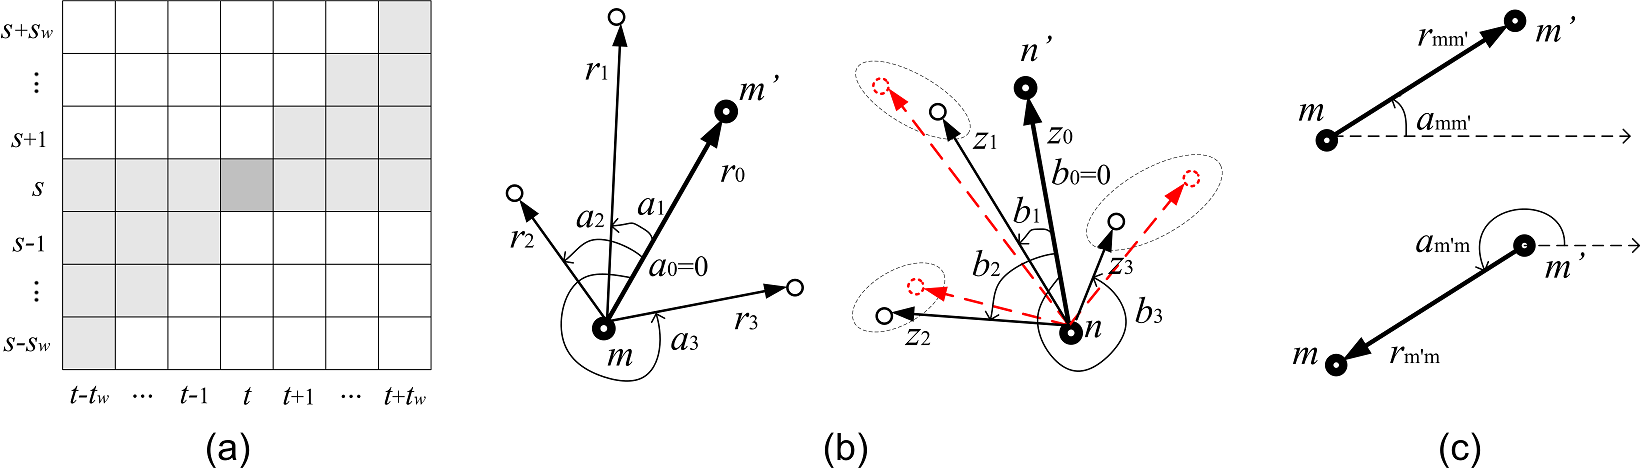
\includegraphics[scale=1.2]{all_illu.png}
\end{center}
\caption{(a) The temporal neighborhood used in to compute (\ref{softvote}). See Section \ref{vote} for details. (b) Illustration of the pairwise pairwise descriptors for groups comprised of three or more participants in the classroom interaction database. See Section \ref{expall} for details. (c) Similar illustrations for groups involving only two participants. See Section \ref{expall} for details.}
\label{all_illu}
\end{figure}

Given the above considerations, two efforts are made in order to allow $W^{*}$ to emerge from the instantaneous matchings $W^{t,s}$'s. First, through metric learning to be presented in Section \ref{MetLearn}, we pursue the effect that the dissimilarity $D(\mathcal{Q}_{t}, \mathcal{D}_{s})$ yields a smaller number if the optimal $N$ agents in $\mathcal{Q}_{t}$ better matches with $\mathcal{D}_{s}$, and yields a larger number otherwise. Second, instead of directly using the dissimilarity scores $D(\mathcal{Q}_{t}, \mathcal{D}_{s})$ for the companion accumulator array, we consider the fact that if the matching $W^{t,s}$ is optimal at time pair $(t,s)$, the optimal matchings at the temporally nearby (input, exemplar) time pairs should be also achieved by the same matrix $W^{t,s}$. This means that the matching matrices of these nearby times should all agree, and their dissimilarities $D$'s should all be small. Therefore, we use the follow temporal-consistency preserved dissimilarity measure to vote in the companion array for $W^{t,s}$
\begin{equation}
\label{softvote}
v(W^{t,s})=\sum_{(t',s')\in\mathcal{N}(t,s)}(\|W^{t,s}-W^{t',s'}\|_{1}+1)D(\mathcal{Q}_{t'}, \mathcal{D}_{s'}).
\end{equation}
Here $\mathcal{N}(t,s)$ is a temporal neighborhood of $(t,s)$ in which we enforce the consistency and it is depicted in Figure \ref{all_illu} (a), where the pair $(t,s)$ is shown in black square and the neighborhood is shown in shaded area. Neighborhood sizes $t_{w}$ and $s_{w}$ are taken as a quarter of the length of a cell on the bottom of the pyramid (See Section \ref{BB})\footnote{When the neighborhood extends out of video boundary, we only consider the cells within the boundary and normalize the vote by the number of cells actually involved.}. (\ref{softvote}) implies that, when evaluating the vote $v(W^{t,s})$ for input time $t$ against exemplar time $s$, we also look at the interactive behavior happening ahead of (resp. after) $t$, and expect that the two aforementioned consistencies are maintained so that the the interactive behaviors happening ahead of (resp. after) $t$ resembles that happening ahead of (resp. after) $s$ in the exemplar, in the sense of a smaller $D$ and a same matching matrix. Eventually, a better matching will receive a lower vote $v$.

\begin{algorithm}
\footnotesize{
\begin{enumerate}
\item Clear both accumulator arrays;
\item For each $t\in[1,T], s\in[1,S]$, increment the count for the matching matrix $W^{t,s}$ by 1, and increase the vote in the\\ 
companion array corresponding to $W^{t,s}$ by $v(W^{t,s})$;
\item Identify a subarray of matrices receiving more than $\frac{S}{2}$ counts, \\
and normalize the dissimilarity votes in the companion subarray 
\\by corresponding counts;
\item Report the matching matrix $W^{*}$ to be the one in the subarray receiving the minimum normalized dissimilarity vote.
\end{enumerate}
}
\caption{\small Voting procedure for identify the participants (\textit{i.e.}, the best matching $W^{*}$).}
\label{Algo:1}
\end{algorithm}

 As a result, the voting procedure is shown in Algorithm \ref{Algo:1}, where in the last two steps we find among those matching matrices which receive a substantial number of supports from instantaneous matchings the best matching $W^{*}$ with the lowest average dissimilarity to the exemplar. This idea is also illustrated in Figure \ref{diagram}, where a thick matching line indicates a strong similarity (low vote $v$), and the agents receiving the average lowest votes are selected as participants.



\subsection{Branch-and-Bound Temporal Localization}
\label{BB}


Once the participants are determined through the best matching $W^{*}$, it is straightforward to recompute the dissimilarities under this specific matching $\hat{D}(\mathcal{Q}_{t}, \mathcal{D}_{s}, W^{*})$, which tells how similar the interaction of the individuals selected by $W^{*}$ at time $t$ is to the exemplar at time $s$, for all $(t,s)$ pairs (See \ref{agg}). We can further get  $D^{*}(t)=\min_{s}\hat{D}(\mathcal{Q}_{t}, \mathcal{D}_{s}, W^{*})$, the minimal dissimilarity of the input interaction by the selected participants to the entire exemplar, as well as $s^{*}(t)=\arg\min_{s}\hat{D}(\mathcal{Q}_{t}, \mathcal{D}_{s}, W^{*})$, the time in the exemplar at which the input at time $t$ exhibits this maximum similarity.  

If in the input between starting time $t_{s}$ and ending time $t_{e}$ ($1\leq t_{s}<t_{e}\leq T$) the selected group of people perform exactly the same interaction as the exemplar (between time $1$ and $S$), what should $D^{*}(t)$ and $s^{*}(t)$ ideally look like in this interval? Obviously, 1) the dissimilarities $D^{*}(t)$'s should be small for $t_{s}\le t\le t_{e}$ and be large for other $t$'s, and 2) the optimally aligned time $s^{*}(t)$ should reside at a similar relative temporal location between $1$ and $S$ as the input time $t$ resides between $t_{s}$ and $t_{e}$.

To realize 1), we use the approach in Section \ref{MetLearn}, where the dissimilarities $D^{*}(t)$ toward zero in the `ground-truth' interval $[t_{s}, t_{e}]$ and toward a large positive number $2\Delta$ otherwise. To formally describe the temporal aligning condition in 2), we employ a temporal pyramid with a total of $L$ levels and $2^{l}$ equal-length cells at the $l$th level to encode the temporal location of a particular time in an interval. Specifically, we define $t\in\mathcal{C}(T_{s},T_{e}, l,i)$ to mean that time $t$ belongs to the $i$th cell at the $l$th level of a $L$-level temporal pyramid on the interval $[T_{s},T_{e}]$, and $s\in\mathcal{C}(1,S, l,i)$ to mean that time $s$ belongs to the $i$th cell at the $l$th level of the pyramid on the interval $[1,S]$. Then, the quantity
\begin{equation}
k(t, T_{s},T_{e}, s, 1,S)\triangleq\sum^{L-1}_{l=0}\sum^{2^{l}}_{i=1} \mathbf{1}(t\in\mathcal{C}(T_{s},T_{e}, l,i))\mathbf{1}(s\in\mathcal{C}(1,S, l,i))
\end{equation}
achieves its maximum if and only if $s$ resides at the same relative temporal location between $1$ and $S$ as $t$ resides between $T_{s}$ and $T_{e}$.

As a result, the function
\begin{equation}
q(t)\triangleq k(t, T_{s},T_{e}, s^{*}(t), 1,S)(D^{*}(t)-\Delta)
\end{equation}
achieves a negative value in the desirable interval $t_{s}\le t\le t_{e}$(because $k(t, T_{s},T_{e}, s^{*}(t), 1,S)$ achieves the maximum positive number and $(D^{*}(t)-\Delta)$ is approximately equal to $-\Delta$), and achieves zero or a positive value otherwise, as illustrated in the lower part of Figure \ref{diagram}. Consequently, the function
\begin{equation}
\label{quality}
f(T_{s}, T_{e})\triangleq\sum^{T_{e}}_{t=T_{s}}q(t)
\end{equation}
achieves the global minimum if and only if the interval $[T_{s}, T_{e}]$ is exactly aligned to the desirable interval $[t_{s}, t_{e}]$. 

The significance of function $f$, is that it satisfied the requirement for the `quality function' studied in \cite{Lampert}, which enables an efficient branch-and-bound search to obtain the optimal solutions for $T_{s}$ and $T_{e}$, instead of a sliding window at multiple scale as required for the majority of existing work. We detail the branch-and-bound algorithm and justify its rationale in the Appendix as supplementary material.


The procedure described in Sections \ref{vote} and \ref{BB} is repeated multiple times for each input video and each exemplar. After we find a best solution of $(W^{*}, T_{s}, T_{e})$, we remove the corresponding tracks in the corresponding interval before we re-execute the same procedure for the second-best solution, and so on. In this way, we obtain multiple responses in the input for each exemplar, and  the input is also matched against multiple database exemplars. In the end, we have for the input video a pool of space-time localizations, with each of these `detected interactions' associated through similarity scores to one or several exemplars. To classify a a detected interaction, we simply apply the majority of the category labels of the top-ranked associated exemplars.


%\subsection{Instantaneous Optimal Matching}
\label{agg}

We now discuss the first step, which serves dissimilarity $\hat{D}(\mathcal{Q}_{t}, \mathcal{D}_{s}, W^{*})$ to the third step, and the score $D(\mathcal{Q}_{t}, \mathcal{D}_{s})$ as well as instantaneous optimal matching $W^{t,s}$ to the second step. Essentially, we seek to compute a dissimilarity between the instantaneous ensembles $\mathcal{Q}_{t}=\{\mathbf{f}_{m,t},\mathbf{g}_{m,m',t}\}$ and $\mathcal{D}_{s}=\{\mathbf{f}^{D}_{n,s},\mathbf{g}^{D}_{n,n',s}\}$. While we will not define them until Section \ref{MetLearn}, suppose for now that there exists an `atomic' distance function $d_{I}(\mathbf{f}_{m,t}, \mathbf{f}^{D}_{n,s}) $ for comparing two individual descriptors $\mathbf{f}_{m,t}$ and $\mathbf{f}^{D}_{n,s}$, as well as another atomic function $d_{P}(\mathbf{g}_{m,m',t}, \mathbf{g}^{D}_{n,n',s}) $ for comparing two pairwise descriptors $\mathbf{g}_{m,m',t}$ and $\mathbf{g}^{D}_{n,n',s}$. We aggregate the overall dissimilarity $\hat{D}(\mathcal{Q}_{t}, \mathcal{D}_{s}, W^{*})$ or $D(\mathcal{Q}_{t}, \mathcal{D}_{s})$ from the atomic distances. Recall that the matching matrix $W\in\mathcal{W}$ encodes which of the input targets is mapped to each of the exemplar agents, and therefore a natural aggregation mechanism is 
\begin{equation}
\begin{split}
&\hat{D}(\mathcal{Q}_{t}, \mathcal{D}_{s}, W)=\\
&\sum_{nm}w_{nm}d_{I}(\mathbf{f}_{m}, \mathbf{f}^{D}_{n})+\sum_{nmn'm'}w_{nm}w_{n'm'}d_{P}(\mathbf{g}_{m,m',s}, \mathbf{g}^{D}_{n,n',t}),
\end{split}
\end{equation}
in which the dissimilarity between two ensembles under a particular matching $W$ is added from all atomic distances between associated pairs.

Consequently, the score $D(\mathcal{Q}_{t}, \mathcal{D}_{s})$ naturally becomes the one from the optimal matching, \textit{i.e.}, the minimum overall dissimilarities $\hat{D}$'s over all possible matching matrices: $D(\mathcal{Q}_{t}, \mathcal{D}_{s})=\min_{W\in\mathcal{W}}\hat{D}(\mathcal{Q}_{t}, \mathcal{D}_{s}, W)$. At the same time, $W^{t,s}=\arg\min_{W\in\mathcal{W}}\hat{D}(\mathcal{Q}_{t}, \mathcal{D}_{s}, W)$ essentially identifies the participants among the input targets which share the maximum similarity with the database exemplar.  Let $\mathbf{w}$ be a long vector by stacking the columns of $W^{t,s}$, the optimization can be expressed as
\begin{equation}
\label{Prob1}
\min_{w_{nm}\in\{0,1\}}\mathbf{c}^{T}\mathbf{w}+\mathbf{w}^{T}H\mathbf{w},\textup{s.t.} W\mathbf{1}=\mathbf{1}, \mathbf{1}^{T}W\leq\mathbf{1}^{T},
\end{equation}
where $\mathbf{c}$ is a $MN\times 1$ vector whose elements come from corresponding individual descriptors $d_{I}(\mathbf{f}_{m,t}, \mathbf{f}^{D}_{n,s})$'s, and $H$ is a $MN\times MN$ matrix whose elements are the corresponding pairwise descriptors $d_{P}(\mathbf{g}_{m,m',t}, \mathbf{g}^{D}_{n,n',s})$'s. As this optimization problem has integer constraints and is generally not convex, we alternatively solve
\begin{equation}
\label{Prob2}
\min_{w_{nm}\in[0,1]}(\mathbf{c}+\hat{\mathbf{c}})^{T}\mathbf{w}+\mathbf{w}^{T}(H+\hat{H})\mathbf{w}, \textup{s.t.} W\mathbf{1}=\mathbf{1}, \mathbf{1}^{T}W\leq\mathbf{1}^{T},
\end{equation}
where $\hat{\mathbf{c}}=[\sigma_{1},\sigma_{2},\cdots,\sigma_{MN}]^{T}$, $\hat{H}=diag\{-\sigma_{1},-\sigma_{2},\cdots,-\sigma_{MN}\}$, and $\sigma_{i}$ is a sufficiently large number satisfying $\sigma_{i}>\sum^{MN}_{j=1,j\neq i}|H_{ij}|+H_{ii}$.

Note that $\hat{H}$ imposes a negative strictly dominant diagonal to $H$ and the quadratic term $\hat{H}+H$ is strictly negative definite. Therefore, (\ref{Prob2}) is a concave programming in the convex unit hypercube $[0,1]^{N\times M}$ and will achieve its minimum at one of the feasible vertices. The feasible vertices, meanwhile, are exactly the feasible solutions of (\ref{Prob1}), and at these vertices, the values of the objective of (\ref{Prob2}) are equal to those of (\ref{Prob1}) due to the cancellation brought by $\hat{\mathbf{c}}$. It is therefore implied that by solving the much more efficient Problem (\ref{Prob2}) we obtain the exact solution for the original Problem (\ref{Prob1}). We solve (\ref{Prob2}) using the CVX toolbox \cite{cvx}.



%% !TEX root =  GroupDet.tex

\section{Descriptor Metric Learning}
\label{MetLearn}
\vspace{-5pt}
As mentioned in Sec. \ref{agg}, we learn matrices $\Sigma_{I}$, $\Sigma_{P}$ for the Mahalanobis distances $d_I(\mathbf{f},\mathbf{f}')$ and $d_P(\mathbf{g},\mathbf{g}')$, so that the learned metrics can: 1) enhance discrimination between exemplar categories by ensuring that distances are smaller when descriptors are drawn from roughly the same temporal location within a labeled exemplar of the same category, and larger otherwise; and 2) enhance the accuracy of temporal localization by ensuring that distances between labeled ensembles and unlabeled ``background'' ensembles are large. The combination of 1) and 2) leads to more accurate spatial localizations of participants (\ie better $W^{*}$ as discussed in Sec. \ref{vote}), and induces the ``quality function'' conditions required for efficient temporal localization by branch-and-bound (Sec.~\ref{BB}). We achieve all of these benefits simultaneously by using an adaptation of the Large Margin Nearest Neighbor (LMNN) framework~\cite{Weinberger:ML}. 

For each application scenario, we use a training set of exemplar videos---possibly having varying numbers of agents $N$---that are annotated with start/end times, category labels, $N$-agent correspondences between exemplars of the same category. We use unlabeled time units in the videos as ``background'' samples. Intuitively, the learned metrics should satisfy the six types of constraints shown in Fig.~\ref{ML_illustration}. This figure depicts three different exemplar videos in which a subset of time units have been labeled as being distinctive interactions of two different classes. In this example, each labeled exemplar is shown as being divided into two cells; these correspond to the lowest level of the temporal pyramid described in Sec.~\ref{BB}. The first three constraints in the list enhance discrimination between categories, while the last three enhance the accuracy of temporal localization. Offsetting all of the distances by $-1$ ensures that the function $q(t)$ in (\ref{qfunction}) assumes proper negative values as required for branch-and-bound search. 

\begin{figure}[t]
\vspace{-5pt}
\begin{centering}
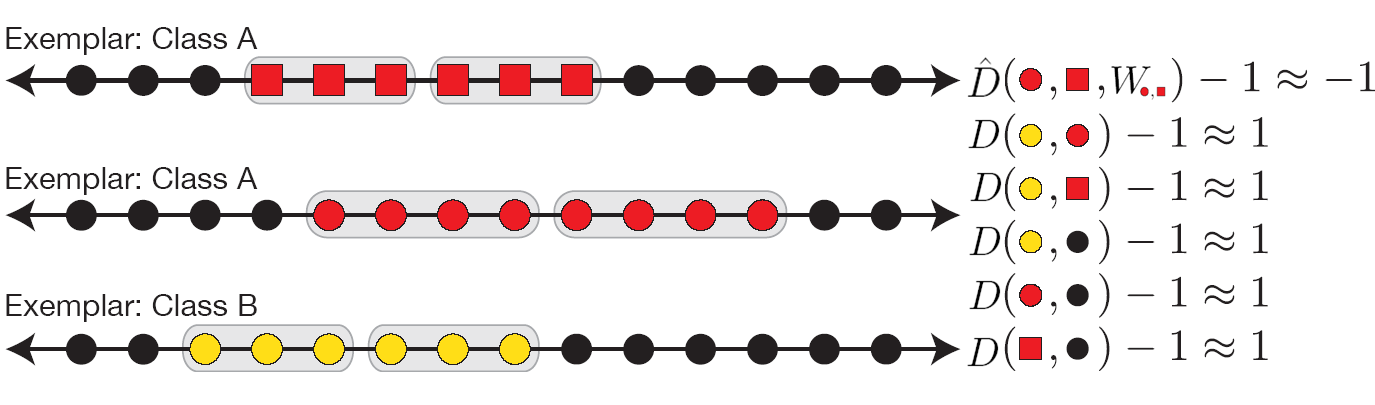
\includegraphics[width=\columnwidth]{MetricLearning_new}
\end{centering}
\caption{Constraints used in discriminative metric learning. Each row is an annotated two-cell exemplar with markers representing instantaneous descriptor-ensembles at each time unit. For discrimination between interaction categories, distances between ensembles of the same class (red circles and red squares) should be small whenever they occur in the same cell number; and distances for different classes (red vs. yellow) should be large. For effective and efficient temporal localization, distances between ensembles at labeled times and unlabeled ``background'' times (black circles) should be large, and all distances should be offset by $-1$. See text for details.}
\label{ML_illustration}
\vspace{-5pt}
\end{figure}

We enforce these constraints through an LMNN framework by construct two collections from our database exemplars. The collection $\mathcal{P}$ contains all pairs of instantaneous interaction ensembles that are of the same category (red circles and red squares in Fig.~\ref{ML_illustration}) and occur roughly in the same temporal location within the interaction instances (\ie, in the same cell of the lowest level of the temporal pyramids), together with their ``ground-truth" matchings. The collection $\mathcal{M}$ is comprised of ordered triples $(h,k,l)$ in which ensemble $h$ is the same category as ensemble $k$ and ensemble $l$ is either of a different category or background. Having defined these two collections, each Mahalanobis metric is found by solving
\begin{equation}
\vspace{-5pt}
\label{classify}
\begin{split}
&\min_{\Sigma_{I}, \Sigma_{P}} \sum_{(u,v)\in\mathcal{P}}\hat{D}(\mathcal{D}_{u}, \mathcal{D}_{v}, W_{u,v})+\gamma\sum_{(h,k,l)\in\mathcal{M}}\xi_{h,k,l},\\
&\textup{s.t.}  \hat{D}(\mathcal{D}_{h}, \mathcal{D}_{l}, W)-\hat{D}(\mathcal{D}_{h}, \mathcal{D}_{k}, W_{h,k})\ge 2-\xi_{h,k,l},\\
& \Sigma_{I}\succeq 0, \Sigma_{P}\succeq 0, \xi_{h,k,l}\ge0,
\end{split}
\end{equation}
where $W_{u,v}$ is the ``ground-truth" matching for pair $(u,v)$ and $W$ is an arbitrary matching in $\mathcal{W}$ \footnote{It is useful to add to the collection $\mathcal{M}$ additional triples in which $l$ is derived from same-category same-cell pairs but with permuted incorrect matching matrices. In this case $\hat{D}(\mathcal{D}_{h}, \mathcal{D}_{l}, W)$ in (\ref{classify}) is replaced by $\hat{D}(\mathcal{D}_{h}, \mathcal{D}_{l}, \bar{W}_{h,l})$, where $\bar{W}_{h,l}$ is the permuted incorrect matching.}. The minimization over either $\Sigma_{I}$ or $\Sigma_{P}$ is exactly a LMNN problem \cite{Weinberger:ML}, and we apply LMNN multiple times to separately learn one distinct pair of ($\Sigma_{I}, \Sigma_{P}$) for each value of $N$ that exists in the training set. 


%Recall that 1) in Section \ref{vote} we expect the score $D$ to be small when a temporal unit in the input is best aligned to a temporal unit in the exemplar by the `correct' matching matrix; and 2) in Section \ref{BB} we expect the dissimilarity $D^{*}(t)$ are driven toward zero in the `ground-truth' interval $[t_{s}, t_{e}]$ , and toward a large positive number $2\Delta$ otherwise. For both purposes, we learn an effective ensemble dissimilarity measure. Recall that the ensemble dissimilarity $D$ or $\hat{D}$ is aggregated from `atomic' descriptor distances $\{ d_{I}(\mathbf{f}_{m,t}, \mathbf{f}^{D}_{n,s}), d_{P}(\mathbf{g}_{m,m',t}, \mathbf{g}^{D}_{n,n',s})\}$, and the ensemble dissimilarity learning therefore narrows down to learning effective `atomic'  distances.  We parameterize an atomic distance by a Mahalanobis metric, \textit{i.e.}, let $d_{I}(\mathbf{f}, \mathbf{f}')=(\mathbf{f}-\mathbf{f}')^{T}\Sigma_{I}(\mathbf{f}-\mathbf{f}')$ and $d_{P}(\mathbf{g}, \mathbf{g}')=(\mathbf{g}-\mathbf{g}')^{T}\Sigma_{P}(\mathbf{g}-\mathbf{g}')$, where $\Sigma_{I}\succeq 0$ and $\Sigma_{P}\succeq 0$ are positive semi-definite matrices.  
%
%We learn each pair of Mahalanobis metrics $(\Sigma_{I}, \Sigma_{P})$ for each number of participants separately. To do so, we construct two different types of collections from our database exemplars. The first collection, $\mathcal{P}$, contains all pairs of instantaneous interaction ensembles that are similar to each other. The second collection, $\mathcal{M}$, is comprised of all ordered triples $(h,k,l)$ in which ensemble $h$ is similar to ensemble $k$ but they two  are dissimilar to ensemble $l$. In the present case, we build the collection $\mathcal{P}$ and the ($(h,k)$-indexed) similar pairs in collection $\mathcal{M}$ using all instantaneous ensemble pairs with their ground-truth matching matrices from the same category extracted from the same cell at the lowest level of the pyramid. Similarly, we include in the ($(h,l)$-indexed and $(k,l)$-indexed) dissimilar pairs of collection $\mathcal{M}$ the ensembles extracted from: 1) different-category exemplars; 2) same-category same-cell ensembles with simulated wrong matching matrices; and 3) ensembles within interaction intervals against ensembles from `background' non-interaction intervals. Eventually, we find the Mahalanobis metrics by solving
%\begin{equation}
%\label{classify}
%\begin{split}
%&\min_{\xi_{h,k,l}\ge0, \Sigma_{I}\succeq 0, \Sigma_{P}\succeq 0} \sum_{(u,v)\in\mathcal{P}}\hat{D}(\mathcal{D}_{u}, \mathcal{D}_{v}, W_{u,v})+\gamma\sum_{(h,k,l)\in\mathcal{M}}\xi_{h,k,l}\\
%&\textup{s.t.}  \hat{D}(\mathcal{D}_{h}, \mathcal{D}_{l}, W_{h,l})-\hat{D}(\mathcal{D}_{h}, \mathcal{D}_{k}, W_{h,k})\ge 2\Delta-\xi_{h,k,l}.
%\end{split}
%\end{equation}
%Note that $\Delta$ is the large positive number as used in (\ref{quality}), and (\ref{classify}) will encourage a similar pair to contribute a negative summand around $-\Delta$ to (\ref{quality}), and encourage a dissimilar pair to contribute approximately $+\Delta$ summand,  thus enabling the branch-and-bound search as introduced in Section \ref{BB}.  The minimization over either $\Sigma_{I}$ or $\Sigma_{P}$ falls into the framework of large margin nearest neighbor (LMNN) formulation \cite{Weinberger:ML}, and we simply decompose (\ref{classify}) into independent LMNN tasks and employ \cite{Weinberger:ML}.

\section{Experiments}
\label{expall}


\noindent\textbf{Classroom Interaction Database.} As mentioned, we have collected and annotated a database of 100 video clips capturing students' behaviors in interactive class sessions. The students are seated but occasionally engaged into small-group discussions. The groups are formed in an ad-hoc manner and vary in geometric configurations. The lengths of the videos vary from one minute to four minutes, and the numbers of individuals varies from six to twenty.We have applied an OpenCV face detector and generated long tracks of the bounding boxes using a combination of OpenCV mean-shift tracking and dominant optical flows. We manually eliminate the false-alarm boxes/tracks and recover (very few) miss-detections when using the video for building ground-truth exemplars, and do not involve manual correction when testing our approach. We have manually identified the participants of all two-person, three-person, and four-person interactions and their exact occurrence intervals. Totally, 254 two-person, 112 three-person, and 16 four-person interactions are annotated. In consultation with education experts, we further divide the two-person interactions into three categories (same row, left-back row v.s. right front row, right-back-row v.s. left-front row), and the three-person interactions into four categories (three people in the same row with two looking left, three people in the same row with two looking right, two people in the back row, two people in the front row)\footnote{It is observed by education experts that students' relative pose and positions strongly modulate their behaviors (\textit{e.g.} see \cite{Crouch:PI}) and consequently under their guidance we categorize the interactions based on students' relative pose and geometric configurations.}. Examples of these patterns are shown in Figure \ref{dataset} (supplementary material). The lengths of these occurrence intervals, meanwhile, range from a few seconds to tens of seconds. The 100 videos arise from five long-lectures, and we adopt a leave-one-lecture-out scheme in partitioning the training (exemplars) and testing (inputs). 

A 4-level pyramid is used and a temporal unit is set at half length of the bottom-level cell. We use a coarse representation of the head pose as the individual descriptor. Specifically, we compute the Histogram of Oriented Gradient (HOG) feature within each temporal unit and each box, and apply nine one-against-all SVMs to estimate the likelihood of a HOG feature belonging to nine head poses (front, left, lower-left, lower-front, lower-right, right, back-right, and back-left). The nine-dimensional likelihood vector  serves as our individual descriptor. Meanwhile, we derive the pairwise descriptor for three or more individuals based on the geometrical configurations of the bounding boxes. As shown in the left panel of Figure \ref{all_illu}(b), where a descriptor of target $m$ relative to target $m'$ among five targets at time $t$ is computed, we compute the distances $r_{i}$'s between all others and $m$, and the relative angles $a_{i}$'s between the connecting vectors and $\overrightarrow{mm'}$, and combine all these geometric quantities into a pairwise descriptor $\mathbf{g}_{m,m',t}$. When computing $\mathbf{g}_{n,n',s}$ in the input (right panel of Figure \ref{all_illu}(b)), we align $\overrightarrow{nn'}$ against $\overrightarrow{mm'}$ and predict the locations of the three individuals (shown in red), and compute the true distances $z_{i}$'s and relative angles $b_{i}$'s by locating the nearest individuals to the predicted locations. This pairwise representation achieves invariance under similarity transforms. For two-person interaction, we simply use the distance and the relative angles against the right horizontal axis (Figure \ref{all_illu}(c)). 

We first look into the computational cost. We replace the optimal matching method with an exhaustive enumeration of all possible matchings. We also apply temporal sliding windows at eight scales ranging from half to twice of the exemplar length, stopping using the remaining scales whenever the current window achieves the same quality function value as the branch-and-bound. We show the average computation time for one match between an exemplar and an input on a 8-core 2.8GHz Macintosh in Table \ref{computecost} (supplementary material), where we see clear savings for the proposed approach.

\begin{figure*}[t]
\begin{center}
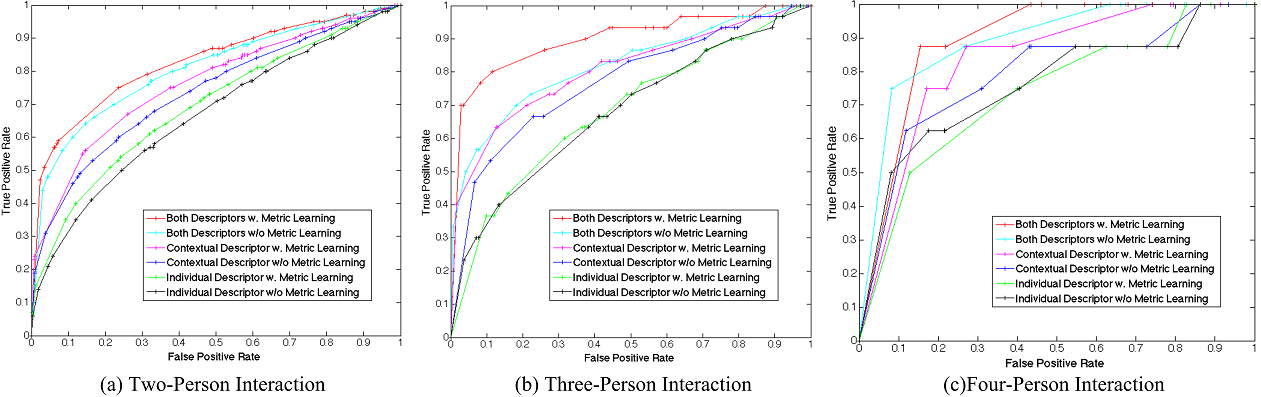
\includegraphics[scale=2.5]{ROC.png}
\end{center}
\caption{ROC curves for identifying the participants of an two-person, three-person, and four-person interactions using the proposed approach and baselines. }
\label{ROC}
\end{figure*}

Note that we combine both individual (pose) descriptor and pairwise (geometric context) descriptor, we then evaluate the effect of this combination by using either descriptor (but not both) and identity matrices as the dissimilarity parameter. The ROC curves for detecting the participants of an interaction is shown in Figure \ref{ROC}. Note that using both descriptors and learning the optimal dissimilarity do yield the best performance, while it is interesting to see that pairwise descriptor performs better than individual descriptor, mainly due to the fact that the interaction only occur among nearby students in a classroom environment and therefore geometric context provides a strong clue for a potential occurrence of interaction. Also note that increased number of participants achieves higher true positives against false positives. This phenomenon is expected, as when more pairwise information is available from more humans, the true interaction pattern is more discriminative against the false ones.

\begin{figure*}[t]
\begin{center}
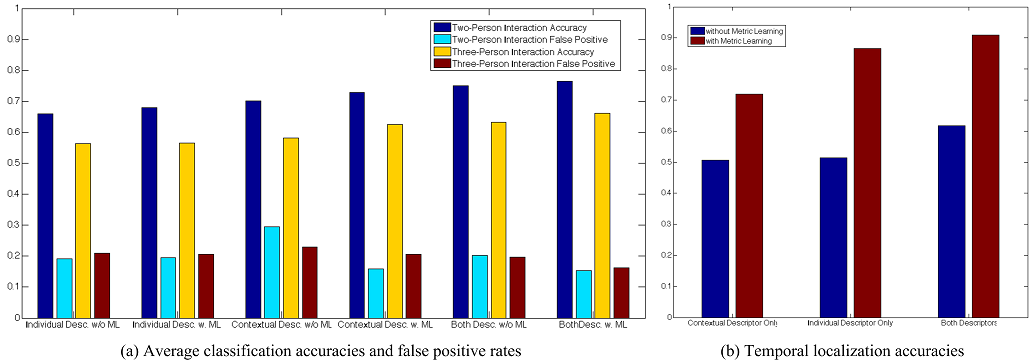
\includegraphics[scale=2.5]{classtemporal.png}
\end{center}
\caption{ Average classification accuracies and false positives for two-person and three-person interactions (Individual and/or pairwise descriptors, with or without metric learning (ML)) and the temporal localization accuracies.}
\label{classtemporal}
\end{figure*}

The third evaluation is on the classification performance for the two-person and three-person interactions (as no further categorization for the four-person interactions is provided, no classification results on four-person interactions are shown). We examine those correctly detected pairs and triples and show the average true positive rates v.s. false positives when further classifying them into the three or four categories in Figure \ref{classtemporal}(a). Again note that either the dissimilarity learning or combining both descriptors gives rise to moderately improvement. As we are at this stage investigating the correctly identified pairs or triples, the head poses serves a stronger evidence than spatial configuration for classification. A pose estimator, which is improved from current coarse representation and is more robust to videos of limited quality, will expect further improved classification performance.

We finally investigate the temporal localization performance. For this purpose, we compute the ratio of the intersection to the union of the estimated interval and the annotated interval, and show the averages in Figure \ref{classtemporal}(b).  Note that the dissimilarity learning is designed in such a way as to encourage the group dissimilarity function to achieves negatives within an activity and positives otherwise. Therefore, the learned quality function of the branch-and-bound search more precisely reflects the boundaries of an activity.

As a visualization, Figure \ref{retrieved} (supplementary material) shows examples of group interaction detection and matching on the classroom interaction database. Note that in the first and third row, a two-person interaction and a three-person interaction are correctly detected and associated with correct exemplars. In the second row, a false positive is detected (shown in blue dashed box), in which the two people are not interacting but demonstrating head poses that are similar to those in a conversation. In the fourth row, the three-person interaction (two looking to the left) is correctly detected but supported by an exemplar of different category (shown in blue dashed box, annotated as `two looking to the right'). Note that the head pose of person marked `2003' appears ambiguous between `looking to the left' and `looking to the right'. In the fifth row, a three-person interaction is correctly identified and associated with correct exemplars, though the head poses of the participants moderately vary among exemplars. 

\vspace{0.05in}

\noindent\textbf{UT-Interaction Dataset.} For a comparison with the state-of-art, we implement our approach on UT-Interaction dataset initially used in \cite{Ryoo:group} and recently again in \cite{Amer:group}. The dataset consists of 20 one-minute videos of continuous executions of 6 classes of two-person interactions: shaking-hands, pointing, hugging, pushing, kicking, and punching. Each video contains at least one instance of every interaction class, where distinct activities may occur at the same time. 10 videos are taken on a parking lot and the other 10 videos are captured in a natural setting by a moving camera. As the UT-Interaction dataset presents simultaneous performance of several activities, activities that may begin and end at arbitrary times, and the presence of people who are not involved in the activity, etc., it is well fitted into the scenario considered here. We follow exactly the same setup as in \cite{Ryoo:group,Amer:group}: 20\% of all available manual segmentations, each occupied by a unique activity instance, are used as `database exemplars' for training. The remaining full (unsegmented) sequences are used for testing. In training, a 4-level pyramid is set up at each ground-truth time interval, and a temporal unit is set at half length of the bottom-level cell. A 32-dimensional histogram of the spatio-temporal features developed by \cite{Dollar:STIP} in each unit and each bounding box is calculated first against a 500-word vocabulary from K-means clustering and then by PCA, and serves as the individual activity descriptor. Another 32-dimensional histogram of the optical flow computed from OpenCV in each unit and each box is calculated against 8 directions and 4 magnitudes, and the difference between the two histograms (relative motion) serves as the pairwise descriptor between the two humans. In testing, we employ the human detector \cite{Pedro:detect}, and associate the detected boxes across frames to form continuous tracks of humans. 

\begin{table}[ht]
\centering \caption{Classification accuracies and false positive (FP) rates for the proposed method and the baselines on UT-Interaction dataset.}
\footnotesize{
\begin{tabular}{|c||c|c|}
\hline   & Accuracy (\cite{Ryoo:group}, \cite{Amer:group}, ours) & FP Rate (\cite{Ryoo:group}, \cite{Amer:group}, ours) \\
\hline Hug &  (0.875, 0.904, \underline{1.00}) & (0.075, 0.055, \underline{0.00}) \\
\hline Kick &  (0.750, 0.775, \underline{0.875})  & (0.138, 0.108, \underline{0.063})\\
\hline Point & (0.625, 0.663,  \underline{0.750}) & (\underline{0.025}, \underline{0.025}, 0.088)\\
\hline Punch & (0.500, 0.632, \underline{0.750})  & (0.201, 0.154,  \underline{0.138})\\
\hline Push & (0.750, \underline{0.782} , 0.750)  & (0.125, \underline{0.101},  0.138)\\
\hline Shake Hands &  (0.750, 0.789, \underline{1.00}) & (0.088, 0.060, \underline{0.00}) \\
\hline\hline Average &  (0.708, 0.758, \underline{0.854})  & (0.108, 0.083,  \underline{0.071})\\
\hline 
\end{tabular}
}
\label{UTaccuFP}
\end{table}


The first interesting investigation is again about the effectiveness of combining both individual descriptor and pairwise descriptor, as well as metric learning for group dissimilarity function. We implement our approach with either but not both descriptor, and without learning the dissimilarity. The performance comparison is show in Table ~\ref{UTaccuFPdegrade} (supplementary material), which again proves the merit of the combined descriptors and learning optimal metrics between descriptors. It is interesting to see the pairwise descriptor plays a more crucial role for this dataset: A significant performance drop arises when we only consider individual action descriptors. The next comparison is against the state-of-art methods \cite{Ryoo:group,Amer:group}. The recognition accuracies and false-alarm rates are shown in Table ~\ref{UTaccuFP}. In this evaluation, we only allow one database exemplar to produce a single response in an input, and claim a true positive only when both the class-label and the identified participants are simultaneously correct, otherwise a false positive is claimed for the exemplar class. We achieve improved accuracy and competitive false positive rate against the baselines. In the third evaluation, we specifically look into the temporal localization and participant identification performance. For temporal localization, we follow exactly the same criterion as in \cite{Amer:group}, requiring a true-positive to achieve both correct classification and a $>50\%$ ratio of the intersection to the union of the estimated interval and ground-truth. we achieve a slightly smaller area under ROC curve than the two baselines, as shown in Table ~\ref{UTarea}. Note that the temporal boundary is essentially ambiguous for these consecutively executed activities. For participant identification, we enforce an even stricter criterion to require $100\%$ correct identification (in contrast to $50\%$ in \cite{Amer:group}) for a true positive, and we outperform \cite{Amer:group}. Note that \cite{Ryoo:group} does not apply human detection and tracking and \cite{Amer:group} does not explicitly operate on the detected bounding boxes. Therefore, our performance should be regarded as an overall effect from both human detection/tracking and our approach.

\begin{table}[ht]
\centering \caption{Area under ROC curve for the proposed method and the baselines on UT-Interaction dataset.}
\footnotesize{
\begin{tabular}{|c|c|c|c|}
\hline   & \cite{Ryoo:group} &  \cite{Amer:group}  &   ours \\
\hline Temporal Localization &  0.91 & \underline{0.94} &  0.89\\
\hline Participants Identification &  N/A & 0.87 &  \underline{0.93}   \\
\hline 
\end{tabular}
}
\label{UTarea}
\end{table}

\vspace{0.05in}

\noindent\textbf{Caltech Resident-Intruder Mouse Dataset.} We also tested the approach on Caltech Resident-Intruder Mouse Dataset \cite{CRIM13}, to demonstrate that our approach can be directly used for a traditional task of temporal segmentation and classification without any changes. The detailed experimental setting and results are presented in the supplementary material.


\vspace{0.05in}

\noindent\textbf{Conclusion.} We have proposed an approach to find small-group interactions in space and time among a larger social clutter. We achieve simultaneous participant identification, temporal localization, and classification. These functionalities are enabled through an effective and efficient integration of multiple modules. Our approach is flexible and generic to various of applications provided that an individual behavior descriptor and a pairwise behavior descriptor are properly given. On the other hand, a further improvement of the overall performance will also rely on the robustness and discrimination of these descriptors, especially when videos are of limited quality such as the classroom videos we use. 


\bibliographystyle{ieee}
{\footnotesize
\bibliography{egbib}
}

\newpage

\newpage

\section{Appendix}

\subsection{Technical Details on the Branch-and-Bound Temporal Localization}
\label{detailBB}

To apply branch-and-bound algorithm to minimize (\ref{quality}), we first specify the spaces where $T_{s}$ and $T_{e}$ may take a value. We denote the length of the shortest exemplar activity as $T_{min}$, then we assume $1\leq T_{s}\leq T-T_{min}+1$ and $T_{min}+1\leq T_{e}\leq T$. Additional constraint may be imposed, such as $T_{min}\leq T_{e}-T_{s}$. Given these information,  the temporal branch-and-bound algorithm, as a companion to the 2-D case studied in \cite{Lampert}, can be derived as in Algorithm \ref{Algo:2}.  In this algorithm, $\hat{f}(T_{s,low}, T_{s,upp}, T_{e,low}, T_{e,upp})$ is a lower bound of the values of the quality function evaluated on all intervals enclosed in $[T_{s,low}, T_{s,upp}]\times [T_{e,low}, T_{e,upp}]$. To calculate this lower bound, we define
\begin{equation}
\begin{split}
&\hat{f}(T_{s,low}, T_{s,upp}, T_{e,low}, T_{e,upp})\\
&=\sum^{L-1}_{l=0}\sum^{2^{l}}_{i=1} \hat{f}(T^{l,i}_{s,low}, T^{l,i}_{s,upp}, T^{l,i}_{e,low}, T^{l,i}_{e,upp})
\end{split}
\end{equation}
where $T^{i,l}_{s}, T^{i,l}_{e}$ are the boundaries of cell $\mathcal{C}(T_{s},T_{e}, l,i)$. In other words, we use the summation of the lower bounds of all cells in the pyramid as the lower bound of the entire interval. The evaluation of $\hat{f}(T^{l,i}_{s,low}, T^{l,i}_{s,upp}, T^{l,i}_{e,low}, T^{l,i}_{e,upp})$, however, is a $\mathcal{O}(1)$ operation with the help of integral dissimilarities $I(t)$ of those negative group dissimilarities $D^{*}(t)$ over $t$. Specifically, let
\begin{equation}
I(t)=\sum^{t}_{t'=1} \min(0,D^{*}(t))
\end{equation}
which only needs to be computed once. Then the lower bound for the cell $\mathcal{C}(T_{s},T_{e}, l,i)$ can be obtained as
\begin{equation}
\hat{f}(T^{l,i}_{s,low}, T^{l,i}_{s,upp}, T^{l,i}_{e,low}, T^{l,i}_{e,upp})=I(T^{l,i}_{e,upp})-I(T^{l,i}_{s,low}).
\end{equation}


\begin{algorithm*}[h]
\begin{enumerate}
\footnotesize{
\item Initialize: Let $T_{s,low}=1$, $T_{s,upp}=T-T_{min}+1$, $T_{e,low}=T_{min}+1$, and $T_{e,upp}=T$; Initialize priority queue $Q$ as empty; 
\item Do
\begin{itemize}
\item If $T_{s,upp}-T_{s,low} \ge T_{e,upp}-T_{e,low}$\\
$T^{(1)}_{s,low}\leftarrow T_{s,low}$, $T^{(1)}_{s,upp}\leftarrow T_{s,low}+\frac{T_{s,upp}-T_{s,low}}{2}$,
$ T^{(1)}_{e,low}\leftarrow T_{e,low}$, $T^{(1)}_{e,upp}\leftarrow T_{e,upp}$,
$T^{(2)}_{s,low}\leftarrow T_{s,low}+\frac{T_{s,upp}-T_{s,low}}{2}$, $T^{(2)}_{s,upp}\leftarrow T_{s,upp}$,
$ T^{(2)}_{e,low}\leftarrow T_{e,low}$, $T^{(2)}_{e,upp}\leftarrow T_{e,upp}$;\\
else \\
$T^{(1)}_{s,low}\leftarrow T_{s,low}$, $T^{(1)}_{s,upp}\leftarrow T_{s,upp}$,
$ T^{(1)}_{e,low}\leftarrow T_{e,low}$, $T^{(1)}_{e,upp}\leftarrow T_{e,low}+\frac{T_{e,upp}-T_{e,low}}{2}$,
$T^{(2)}_{s,low}\leftarrow T_{s,low}$, $T^{(2)}_{s,upp}\leftarrow T_{s,upp}$,
$ T^{(2)}_{e,low}\leftarrow T_{e,low}+\frac{T_{e,upp}-T_{e,low}}{2}$, $T^{(2)}_{e,upp}\leftarrow T_{e,upp}$;
\item If $T_{min}\leq T^{(1)}_{e,upp}-T^{(1)}_{s,low}$,
push $(T^{(1)}_{s,low}, T^{(1)}_{s,upp}, T^{(1)}_{e,low}, T^{(1)}_{e,upp},\hat{f}(T^{(1)}_{s,low}, T^{(1)}_{s,upp}, T^{(1)}_{e,low}, T^{(1)}_{e,upp}))$ into $Q$;\\
\item If $T_{min}\leq T^{(2)}_{e,upp}-T^{(2)}_{s,low}$,
push $(T^{(2)}_{s,low}, T^{(2)}_{s,upp}, T^{(2)}_{e,low}, T^{(2)}_{e,upp},\hat{f}(T^{(2)}_{s,low}, T^{(2)}_{s,upp}, T^{(2)}_{e,low}, T^{(2)}_{e,upp}))$ into $Q$;\\
\item Let $(T_{s,low}, T_{s,upp}, T_{e,low}, T_{e,upp})$ be the tuple in $Q$ achieving the minimal $\hat{f}$;
\end{itemize}
Until $T_{s,low}=T_{s,upp}, T_{e,low}=T_{e,upp}$.
\item Output: $T_{s}\leftarrow T_{s,low}, T_{e}\leftarrow T_{e,low}$. 
}
\end{enumerate}
\caption{\small Branch-and-bound search for temporal localization.}
\label{Algo:2}
\end{algorithm*}

\subsection{Additional Experiments Results}

\subsubsection{Classroom Interaction Database}

\begin{figure}[h]
\begin{center}
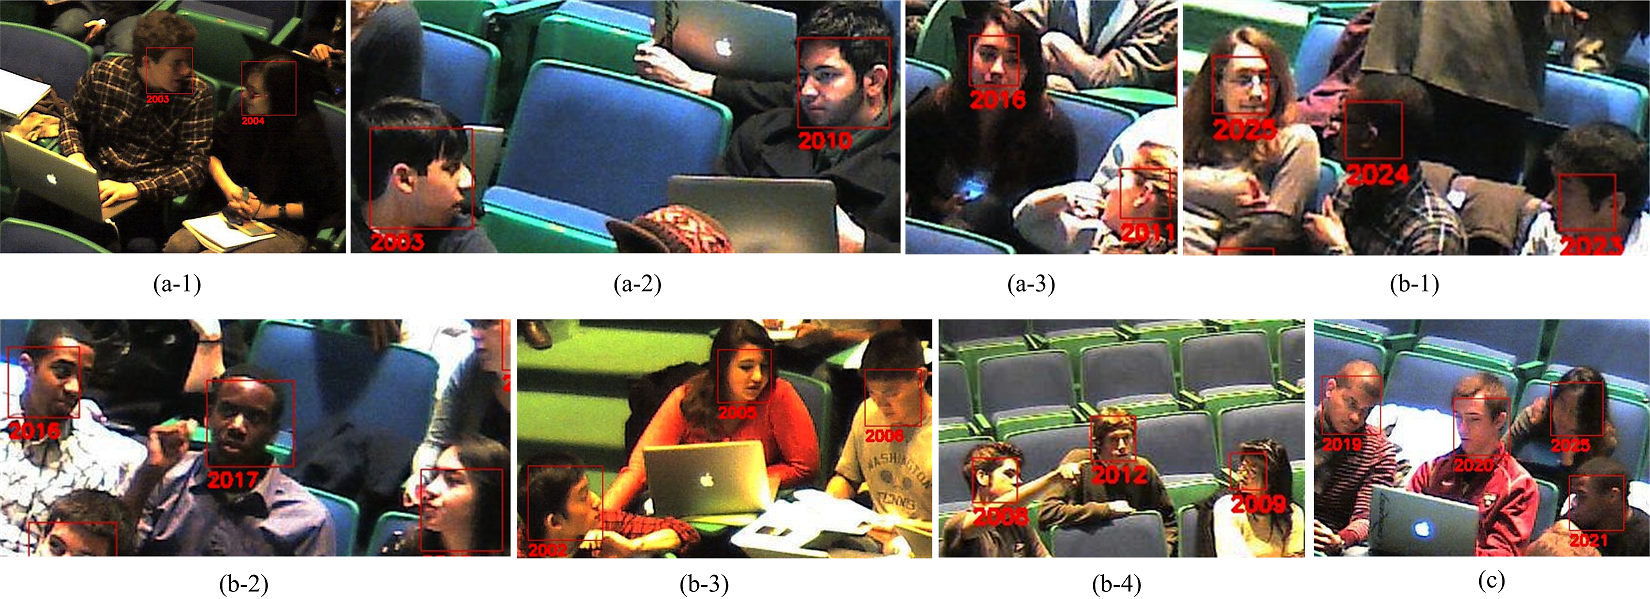
\includegraphics[scale=1.2]{dataset.png}
\end{center}
\caption{Samples of two-person ((a-1)(a-2)(a-3)), three-person ((b-1)(b-2)(b-3)(b-4)), and four-person (c) interactions in the classroom interaction dataset we collected.}
\label{dataset}
\end{figure}

\begin{table}[h]
\centering \caption{Computational cost comparison for the proposed matching approach and baselines (in seconds).}
\footnotesize{
\begin{tabular}{|c|c|c|c|}
\hline    \# of Participants &  2  &  3  &  4   \\
\hline   Exhaustive+Sliding Window & 17.2   & 60.4   & 253.2   \\
\hline  Exhaustive+Branch and Bound &  12.6 &  27.6  &   59.7 \\
\hline  Optimal Pairing+Sliding Window & 12.4  & 23.2   &  40.8  \\
\hline  Proposed & 8.0  &  19.8  &  32.3  \\
\hline 
\end{tabular}
}
\label{computecost}
\end{table}

\begin{figure*}
\begin{center}
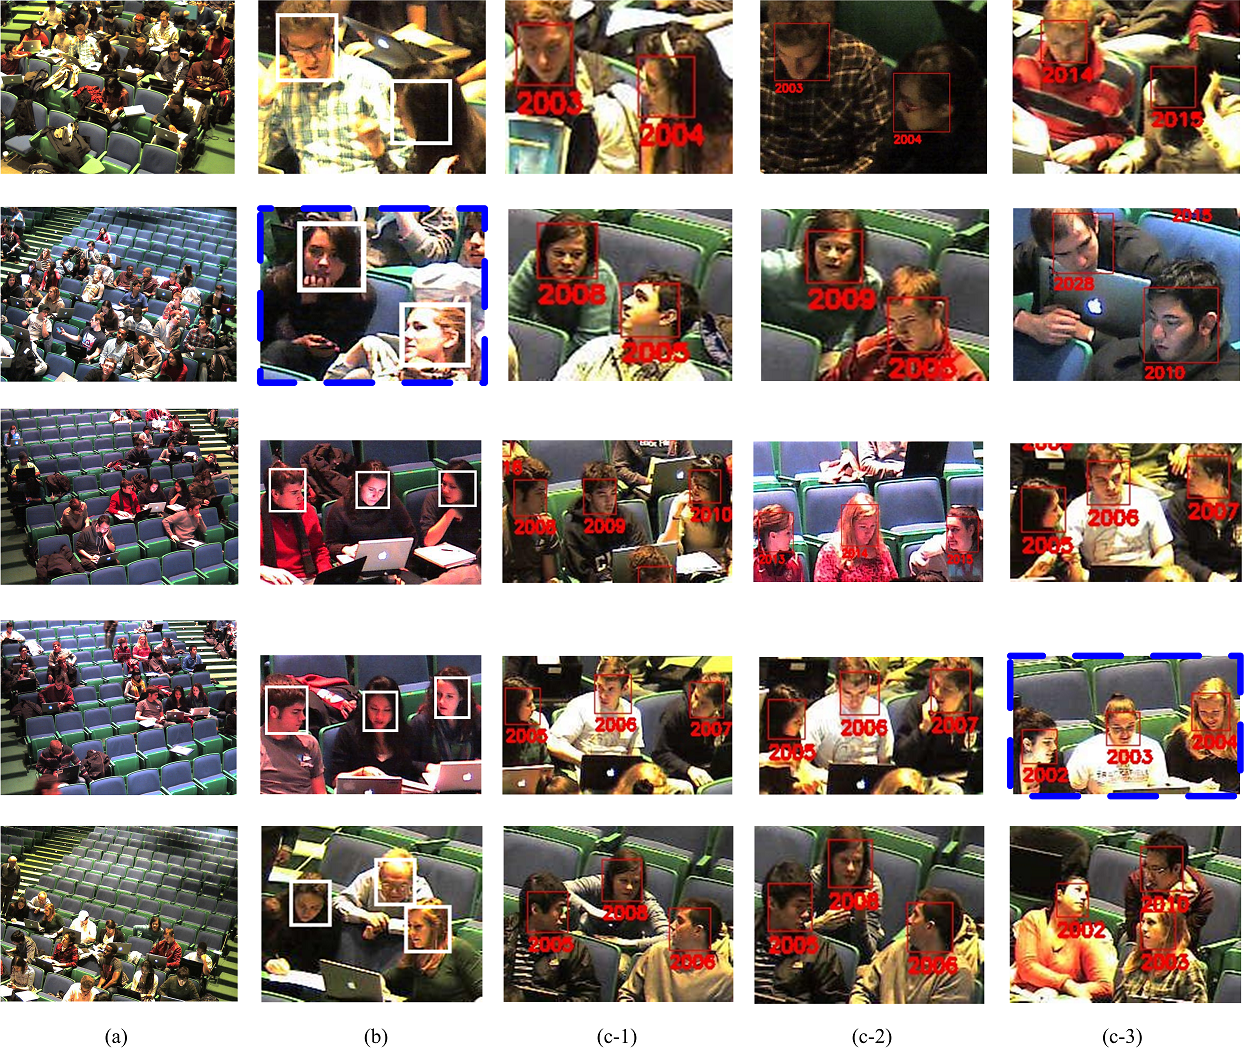
\includegraphics[scale=2.25]{retrieved.png}
\end{center}
\vspace{-10pt}
\caption{Examples of social interaction detection and matching on the classroom interaction database. Each row is an example of detecting a salient interaction from an input and enumerating similar database exemplars: (a) is the input, (b) is the detected social interaction, and (c-1) to (c-3) are the top three associated database exemplars that support this detection.}
\label{retrieved}
\end{figure*}

\subsubsection{UT-Interaction Dataset}


\begin{table}[h]
\centering \caption{Classification accuracies and false positive (FP) rates comparison on UT-Interaction dataset for evaluating the effectiveness of different components of the proposed approach: Individual and/or pairwise descriptors, with or without metric learning (ML).}
\footnotesize{
\begin{tabular}{|c|c|c|c|}
\hline   & Individual only & pairwise only & Both \\
\hline Accur. w. ML & 0.688 & 0.813 & 0.854  \\
\hline Accur. w/o ML & 0.647 & 0.750 & 0.771    \\
\hline FP Rate w. ML &  0.125 & 0.096 & 0.071  \\
\hline FP Rate w/o ML & 0.163 & 0.113 & 0.083\\
\hline 
\end{tabular}
}
\label{UTaccuFPdegrade}
\end{table}


\subsubsection{Caltech Resident-Intruder Mouse Dataset.} 

We also tested the approach on Caltech Resident-Intruder Mouse Dataset \cite{CRIM13}, which contains long video sequences recording pair-wise interactions between two mice. Behaviors are categorized into 12 different mutually exclusive action types, plus an `other' category indicating no behavior of interest is occurring. A video typically lasts around 10 minutes at 25fps with a resolution of 640x480 pixels. Every video frame is labeled with one of the thirteen ground-truth categories, resulting in a segmentation of the videos
into action intervals. For more details please refer to \cite{CRIM13}. Note that in all videos are pair-wise interactions, and our experiment on this dataset is not meant to distinguish the participants, but to demonstrate that our approach can be directly used for a traditional task of temporal segmentation and classification without any changes.

We exactly follow the training/testing partitions provided by the dataset. We extract the spatio-temporal interest points (STIP) based appearance features and compute trajectory-based features from the tracks provided with the dataset as \cite{CRIM13} does (See \cite{CRIM13} for details). Differently from \cite{CRIM13}, we only compute STIP based features inside the bounding boxes enclosing the mice. The trajectory-based features consists of those describing the motion of each individual mouse and those describing the relative motion between two mice. We denote the former as T\_ind and the latter as T\_pair. Again we use a 4-level temporal pyramid, in which the STIP based appearance features are computed as \cite{CRIM13} does and the trajectory based features are also transformed into histograms against 64 codewords. 

Three combinations of features were attempted in \cite{CRIM13}: Trajectory only, STIP only, and using both. For the case trajectory only, our approach has two possible working modes: Using all trajectory-based features as individual descriptors (denoted as Trajectory\_1), or using T\_ind as individual descriptors and using T\_pair as pairwise descriptors (denoted as Trajectory\_2). In the case of STIP only, all features are used as individual descriptors, and in the case of using both, STIP features and trajectory-based features serve as individual descriptor and pairwise descriptors respectively. To classify a segment responded by one or more exemplars, we simply give it the label of the top-ranked exemplar. We follow the same error metric as \cite{CRIM13}, the frame-wise accuracy, and report the results in Table \ref{CRIMAccu}, where it is evident that motion trajectory is much more discriminative than local STIP based features given little articulation in a constrained environment. The competing performance by approach is achieved by splitting the motion into individual ones and pairwise ones and learning separate metrics for them (Trajectory\_2). In other cases, multi-level adaboost based approach exhibits superiority on frame-wise classifications (as in \cite{CRIM13}).


\begin{table}[h]
\centering \caption{Accuracies for the proposed method and the baselines on Caltech Resident-Intruder Mouse Dataset. (\%)}
\footnotesize{
\begin{tabular}{|c||c|c|c|c|}
\hline   & Trajectory\_1  & Trajectory\_2 & STIP & Both \\
\hline \cite{CRIM13} w/o. context & 52.3  & 52.3 & 29.3 & 53.1\\
\hline \cite{CRIM13} w. context &  \underline{58.3} & 58.3 & \underline{43.0} & 61.2\\
\hline Ours w/o. ML &  45.6 & 49.4 & 18.8 & 50.9 \\
\hline Ours w. ML & 54.5 & \underline{66.0} & 31.7 & \underline{62.9}\\
\hline 
\end{tabular}
}
\label{CRIMAccu}
\end{table}

It is observed in \cite{CRIM13} that accuracy varies with the length of the interaction and with the length of window within which the local feature is computed. To investigate the performance of our approach on different lengths of the interaction as compared to \cite{CRIM13}, we implemented the approach in \cite{CRIM13} using trajectory-based features and one-level auto-context classifier. As shown by the result in Figure \ref{frame_no}, our approach is particularly better at localizing longer interactions though \cite{CRIM13} demonstrates its advantage under a shorter feature window on shorter interactions. 

\begin{figure}[h]
\begin{center}
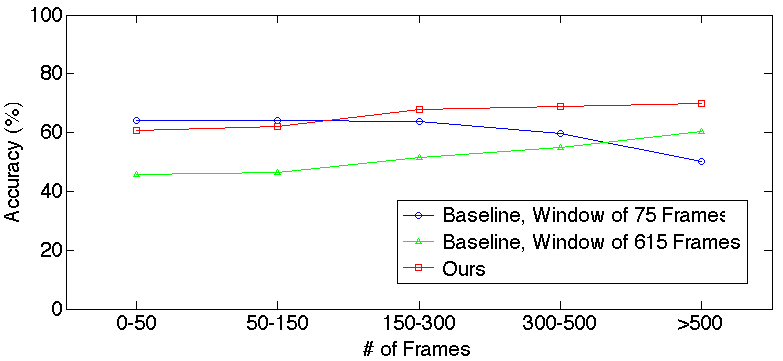
\includegraphics[scale=0.25]{frame_no.png}
\end{center}
\caption{Accuracy comparison for varying length of interactions between \cite{CRIM13} and our approach.}
\label{frame_no}
\end{figure}







\end{document}
